\chapter{Intelligent Grid}

\section {Description}

The network design follows the industry tendency of mixing different types of networks, thus extending their functionality and reliability.
For this reason, it is targeted towards the "smart" home, an environment that the intelligent system is meant control. The standard
approach however, fails to account for an important component in the network - the PC. Formerly neglected by ambient intelligence systems,
the PC is currently the linchpin of the multimedia ambient concepts, such as Microsoft Media Center, Apple FrontRow and HP Digital 
Entertainment Center. When it is in use, the general purpose computing system acts as both a sensor-actuator pair, controlling the network,
as well as a source of computational power for the system to use, reducing overall power consumption \cite{95}.

The `intelligent grid` is the nomenclature for a collection of sub-components belonging to a multitude of fields regarding ambient intelligence,
complementing each others ??. Those components are the derived from sensor networks, providing the ability to monitor and automate processes,
multimedia networks, providing a plethora of I/O, storage and DSP capabilities, and classical computational networks, providing high performance
computing from low cost components. All those parts are combined into a grid network, as it derives computational power most efficiently
\cite{3, 8, 9, 19, 30, 32, 33, 38}.

Based on the definition of ambient intelligence, it can be derived that the intelligent grid can be characterized by the following:
\begin{itemize}
    \item the great majority of technology is embedded, hidden in the background 
    \item is sensitive, adaptive, and responsive to the presence of people and objects 
    \item that augments activities through smart non-explicit assistance 
    \item that preserves security, privacy and trustworthiness while utilizing information when needed and appropriate 
    \item it can accept explicit targeted tasks from the users 
    \item it searches for computational power, being able to provide such a feature. 
\end{itemize}

Stemming from those characteristics, the base schematic of the network can be presented:

\begin{figure}[H]
	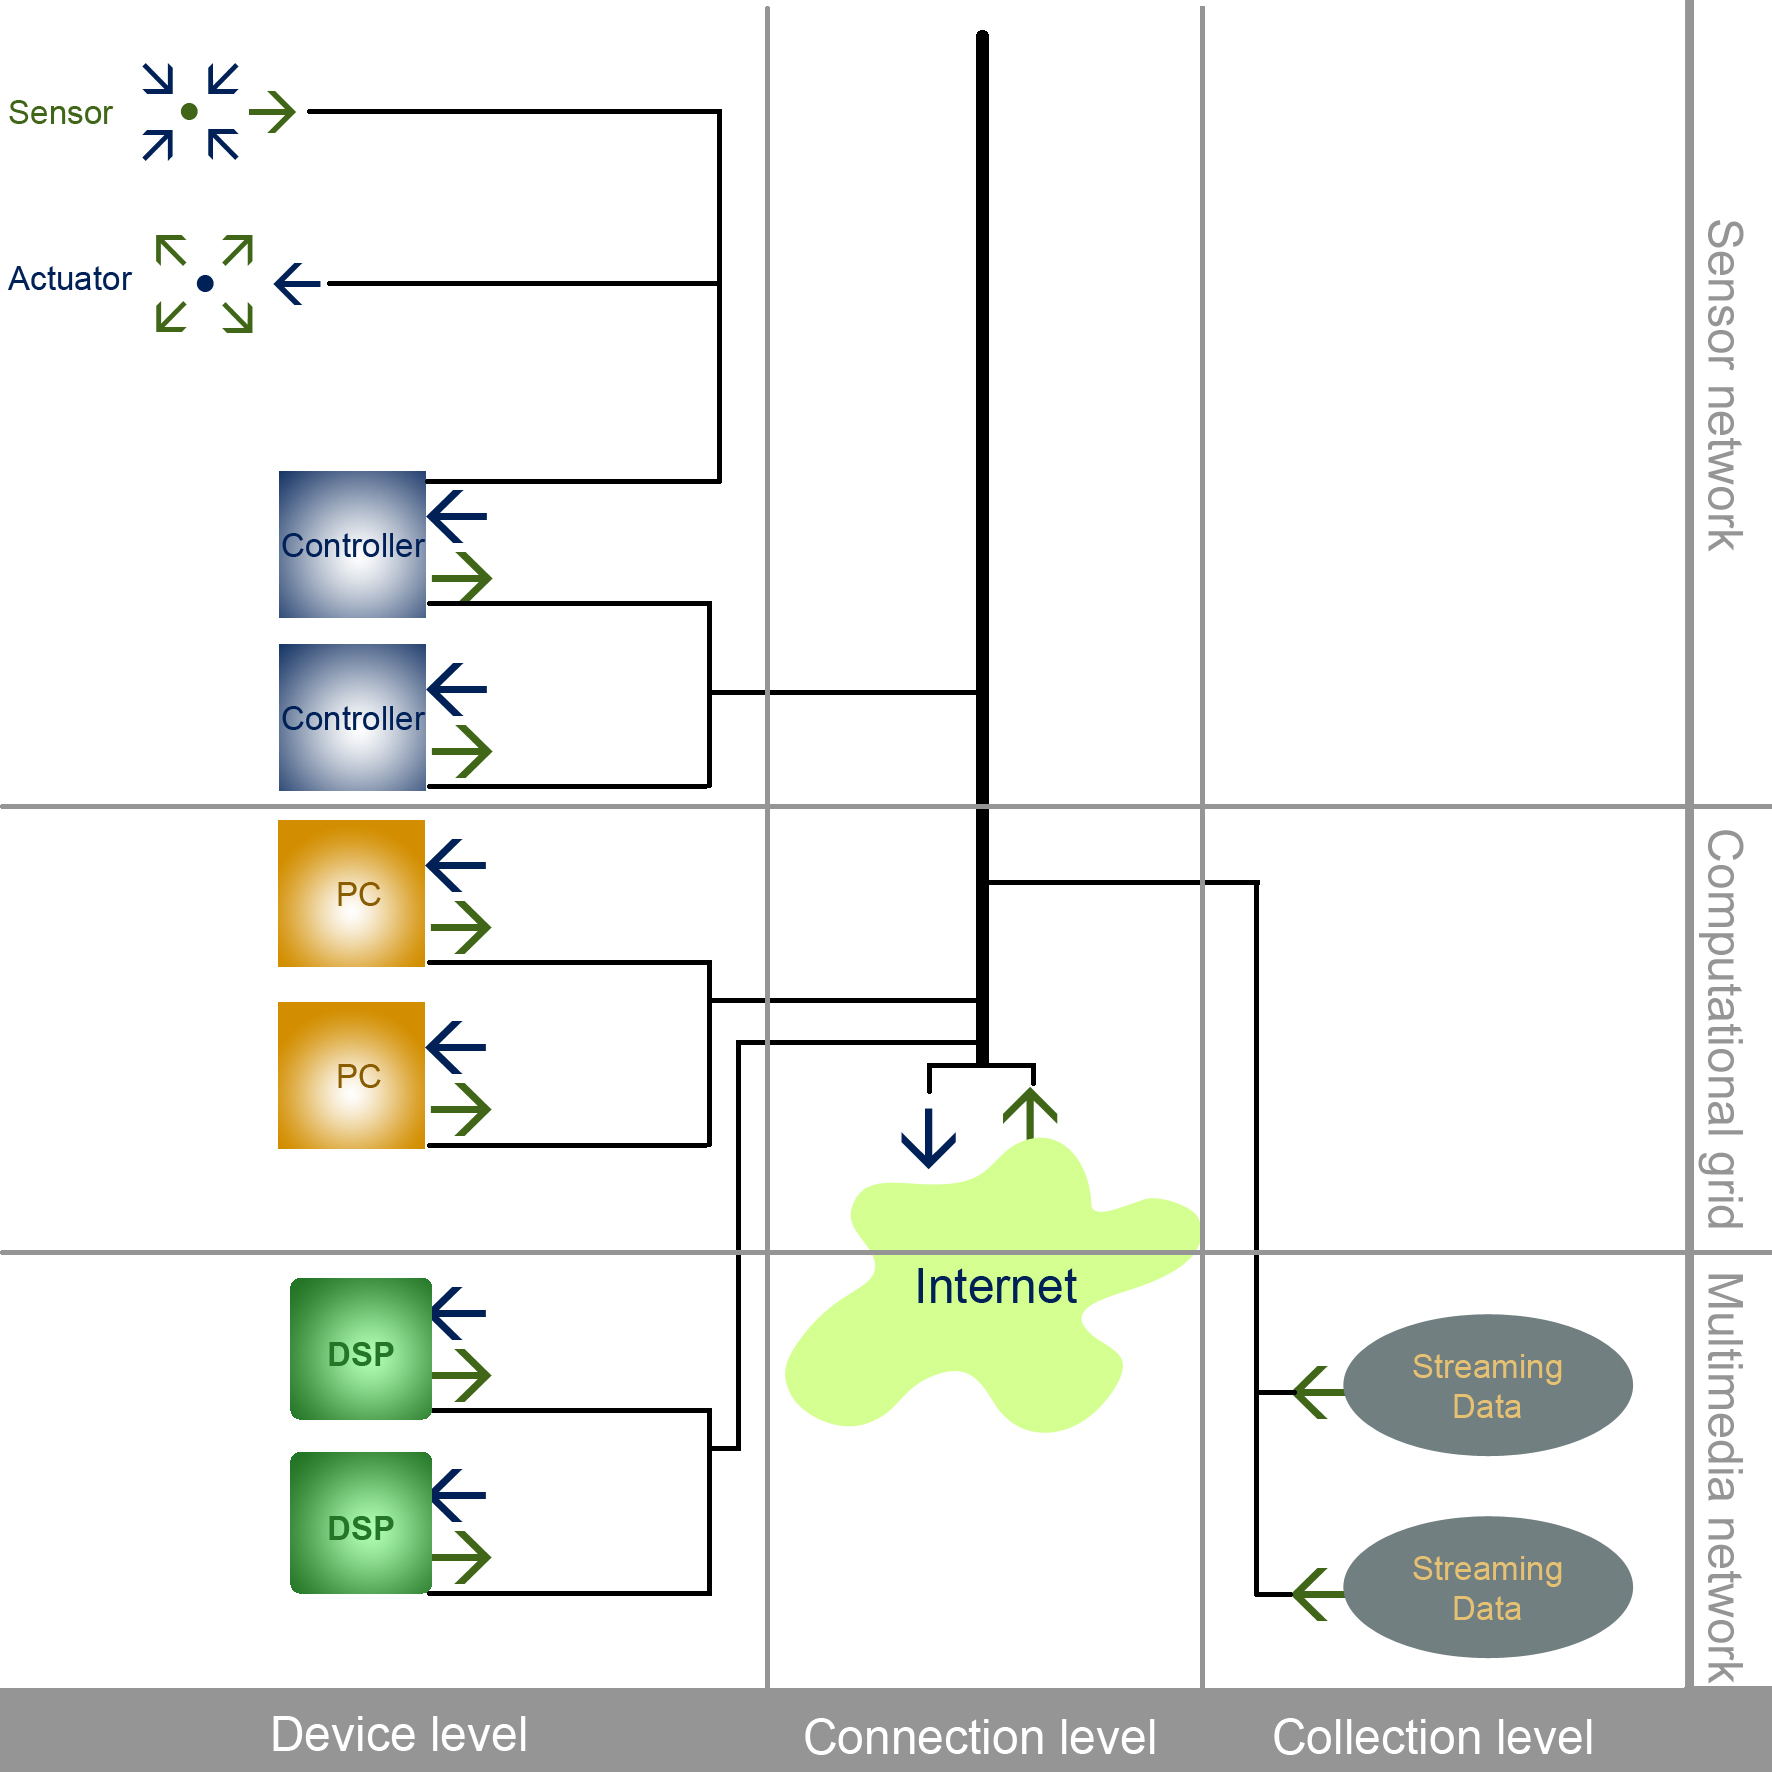
\includegraphics[width=0.9\textwidth, height=0.65\textwidth]{Pic2}
    \caption{The intelligent grid. \cite{88} \label{fig:intelligentGrid}}
\end{figure}

Each sub-network, abstraction level, and its respective equipment is showcased in \cref{fig:intelligentGrid}. Physical components, such as
sensors, actuators, DSPs and PCs are located at device level, with the higher abstraction data storage and streaming are denoted by the
collection level. In between them, handling communication between the devices, as well as linking to the internet, is the connection level.

Due to all of the individual network components involved, the following table presents a comparison between the intelligent grid and 
previous network systems. It can be noted that it encompasses elements form all other networks, resulting in its ability to perform 
computations at the same time as it manages ambient intelligence.

\begin{longtable}[H]{|p{2cm}|p{2cm}|p{3cm}|p{2cm}|p{2cm}|}
	\hiderowcolors
	\caption{Comparison of networks \cite{89}\label{tb:networkComparison}} \\
	\hline
    Network Grid & Sensor grid & Ambient intelligence & Multimedia grid & Intelligent grid  \\
	\hline
	\endfirsthead

	\hline
    \multicolumn{5}{|p{2cm}|}{Continuation of Table \cref{tb:networkComparison}} \\
	\hline
    Network Grid & Sensor grid & Ambient intelligence & Multimedia grid & Intelligent grid  \\
	\hline
	\endhead

	\hline
	\endfoot

	\hline\hline
	\endlastfoot
	\showrowcolors

	\hline
    Sensor Network      & X & X &   & X \\
	\hline
    Multimedia Network  &   & X & X & X \\
	\hline
    Computation Network & X &   & X & X \\
\end{longtable}

It is required that the network is designed for reliability, such as to ensure no errors occur when accessing resources or communicating
between nodes. For this reason, each individual challenge present in ambient intelligence will be presented in regard to the intelligent 
grid, with specific solutions put forward in order to ensure a reliable design. Such a mechanism is represented by the ``consensus issue``,
an approach that is not a subject of this thesis, but is extensively covered in Versavia Ancusa's PhD report \cite{107}.

\section{Power, cost and size analysis}

This approach is taken due to the nature of the hardware being used, such as sensors, actuators, controllers and DSPs, becoming 
"disappearing electronics", meaning super low-power devices that need to rely on a micro-generator instead of a battery for optimal
functionality. Thus the need arises for components that can produce their own energy from ambient sources, called scavenging deceives.
Such solutions are already available, most know being the harvesting of solar energy, but other sources are being covered, some relying 
on temperature, pressure, and even vibration gradients. Currently the idea of energy harvesting is being considered from a system point
of view, pushed by real industrial results, such as the parity between the current electrical grid and solar generated power 
 \cite{36, 70, 71, 94}.

One such developing area is that of nanogenerators, such as nanoscale thermoelectric harvesting (based on the Seebeck effect), and
nanopiezotronics (converting mechanical energy into electricity). Such systems are being developed in the field of MEMS 
(micro-electrico-mechanical systems) in order to converd nanoscale mechanical energy into electrical impulses through the use of
zinc nanowires and a series of electrodes, producing electricity when the wires brush against the electrodes under sufficient vibration.
\cite{23, 71}

Other products, such as the battery-free wireless switches provided by `Lightning Switch` and `Ad Hoc Electronics` convert the button press
into electrical potential. At the same time, battery-free tire sensors are being developed, powered by the impact acceleration converted
through cymbal transducers. \cite{36}

With all other bases covered, the only grid component left to be analyzed from a power, cost and size perspective is the PC, a component
that expected to disappear, in favor of a more streamlined user experience. It is expected that future computers will provide only a basic
interface, with the bulk of the computation being done on cloud infrastructure instead. \cite{13}

\section{Portability, scalability and configurability analysis}

Those factors need to bbe accounted for because changing the application involves software changes, meaning that significant logistical
errors can occur. The proposed solution is to raise the abstraction level \cite{38}:

\begin{figure}[H]
	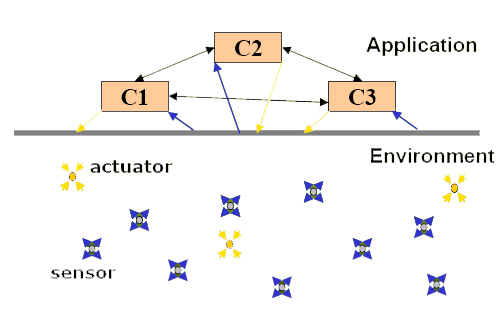
\includegraphics[width=0.9\textwidth, height=0.65\textwidth]{Pic3}
    \caption{Raising abstraction level. \cite{38} \label{fig:abstractionLevel}}
\end{figure}

Derived from \cref{fig:abstractionLevel}, an increase in abstraction level in the case of, for example, the sensor network, involves the
management of individual nodes as a set of computational functions, with the cooperation between them being ensured by a series of sensors
and actuators.

\subsection{Middleware}

Because of the myriad of computer systems running different operating systems and software tools, middleware is a required abstraction
layer meant to provide a common end-point for a distributed heterogeneous system, in order to manage any increase in complexity.

\begin{figure}[H]
	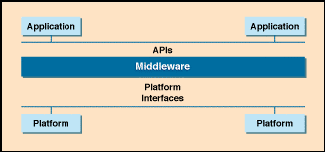
\includegraphics[width=0.9\textwidth, height=0.35\textwidth]{Pic4}
    \caption{Middlewre layer. \cite{72} \label{fig:middleware}}
\end{figure}

Middleware acts as a bridge between individual platform interfaces and higher level APIs, as presented in \cref{fig:middleware}, thus it needs
to support compatibility with both neighboring layers. With the intelligent grid being comprised of three sub-networks, each of their 
requirements must be handled specifically:

\begin{longtable}[H]{|c|c|c|c|}
	\hiderowcolors
	\caption{Overview of the programming requirements \cite{89}\label{tb:programmingRequirements}} \\
	\hline

    \multirow{2}{*}{Programming requirements} & \multicolumn{3}{c|}{Networks based on} \\
    \cline{2-4}
    &Sensor & Multimedia & Computation \\
	\hline
	\endfirsthead

	\hline
    \multicolumn{4}{|c|}{Continuation of Table \cref{tb:programmingRequirements}} \\
	\hline

    \multirow{2}{*}{Programming requirements} & \multicolumn{3}{c|}{Networks based on} \\
    \cline{2-4}
    &Sensor & Multimedia & Computation \\
	\hline
	\endhead

	\hline
	\endfoot

	\hline\hline
	\endlastfoot
	\showrowcolors

    Concealed issues & hardware and distribution & hardware & distribution \\
	\hline
	\hline

    \multicolumn{4}{|c|}{Restricted Resources} \\
	\hline
    Energy                  & X &   &   \\	
	\hline
    computing power         & X & X & X \\	
	\hline
    communication bandwidth & X & X & X \\
	\hline

    Network Dynamics & high & medium & low \\
	\hline

    Scale of Deployments & N*(100…1000) & N*(10…100) & N*(10…100) \\
	\hline
	\hline

    \multicolumn{4}{|c|}{Real-world Integration} \\
	\hline
    Time scale      & X & X & X \\
	\hline
    Location scale  & X & X &  \\
	\hline
	\hline
    \multicolumn{4}{|c|}{Collection and Processing of Data}\\
	\hline
    Preprocessing       & X & X &  \\
	\hline
    Aggregating data    & X & X & X \\
	\hline
    Local processing    &   & X & X \\
	\hline
\end{longtable}

With \cref{tb:programmingRequirements} presenting the requirements for each type of network, the following table showcases how existing types
of middleware can be used for each type of sub-network in the system:

\begin{longtable}[H]{|c|c|c|c|}
	\hiderowcolors
	\caption{Types of middleware and their usage \cite{90} \label{tb:middlewareUsage}} \\
	\hline

    \multirow{2}{*}{Type of aproach} & \multicolumn{3}{c|}{Networks based on} \\
    \cline{2-4}
    &Sensor & Multimedia & Computation \\
	\hline
	\endfirsthead

	\hline
    \multicolumn{4}{|c|}{Continuation of Table \cref{tb:middlewareUsage}} \\
	\hline

    \multirow{2}{*}{Type of aproach} & \multicolumn{3}{c|}{Networks based on} \\
    \cline{2-4}
    &Sensor & Multimedia & Computation \\
	\hline
	\endhead

	\hline
	\endfoot

	\hline\hline
	\endlastfoot
	\showrowcolors

    Events                      & X &   &   \\
	\hline
    Remote Procedure Call       &   & X & X \\
	\hline
    Object Request Broker       &   & X & X \\
	\hline
    Message-oriented            &   &   & X \\
	\hline
    Databases                   & X & X &   \\
	\hline
    Mobile (Intelligent) Agents & X & X & X \\
	\hline
\end{longtable}

As seen in \cref{tb:middlewareUsage}, the most versatile type of middleware is that of "intelligent agents", independent system components
that communicate with each other on a peer to peer basis. The concept of agents stems from the application of artificial intelligence 
to the field of distributed systems - Agent-Oriented Programming (AOP). The most widespread agent oriented middleware is the Java Agent 
Development framework (JADE), a completely distributed middleware system that supports easy extension via additional modules. The framework 
facilitates the development of complete agent-based applications by means of a run-time environment implementing the life-cycle support 
features required by agents, the core logic of agents themselves, and a rich suite of graphical tools. \cite{24}

Being build in Java, JADE benefits form a myriad of third-party libraries, as well as basic language features, making it easily extensible,
while also allowing for other abstraction layers to be build on top of it. Another significant advantage is that JADE is a fully open source
project, adhering to FIPA specifications and IEEE standards.

\subsection{Intelligent Agents}

As a newly emerging technology, agent-based software solutions are at the forefront of scientific research, with significant effort put into
commercial applications of the concept. Agents are, in essence, software components that can operate independently and can be linked together
in order to increase each others capabilities. While single-agent systems can exist, the strength of the system derives from several agents
exchanging messages, through specified protocols, in a collaborative manner. This communication enables coherency between the actions of all
agents in the system, leading to more efficient workflow across the entire network \cite{24, 105}.

Multi-agent systems are already being used in a myriad of applications, from personal use to mission-critical industrial applications, such
as process control, system diagnostics, manufacturing, logistics and network management. All agents are designed to be autonomous and reactive,
meaning that they can operate without human intervention and adapt to changes in their environment. Other characteristics include proactivity, 
for agents that take goal-directed initiative in order to fulfill its function, and mobility, in the case of agents that are able to travel
to different nodes in the network. Each agent can function as standalone applications, resource managers, network services and even APIs for
lower level components. Those characteristics allow for the grid components, such as the controllers, DSPs and PCs, to be considered agents.
Applying the concept of intelligent agents to the design from \cref{fig:intelligentGrid} leads to the following schematic:

\begin{figure}[H]
	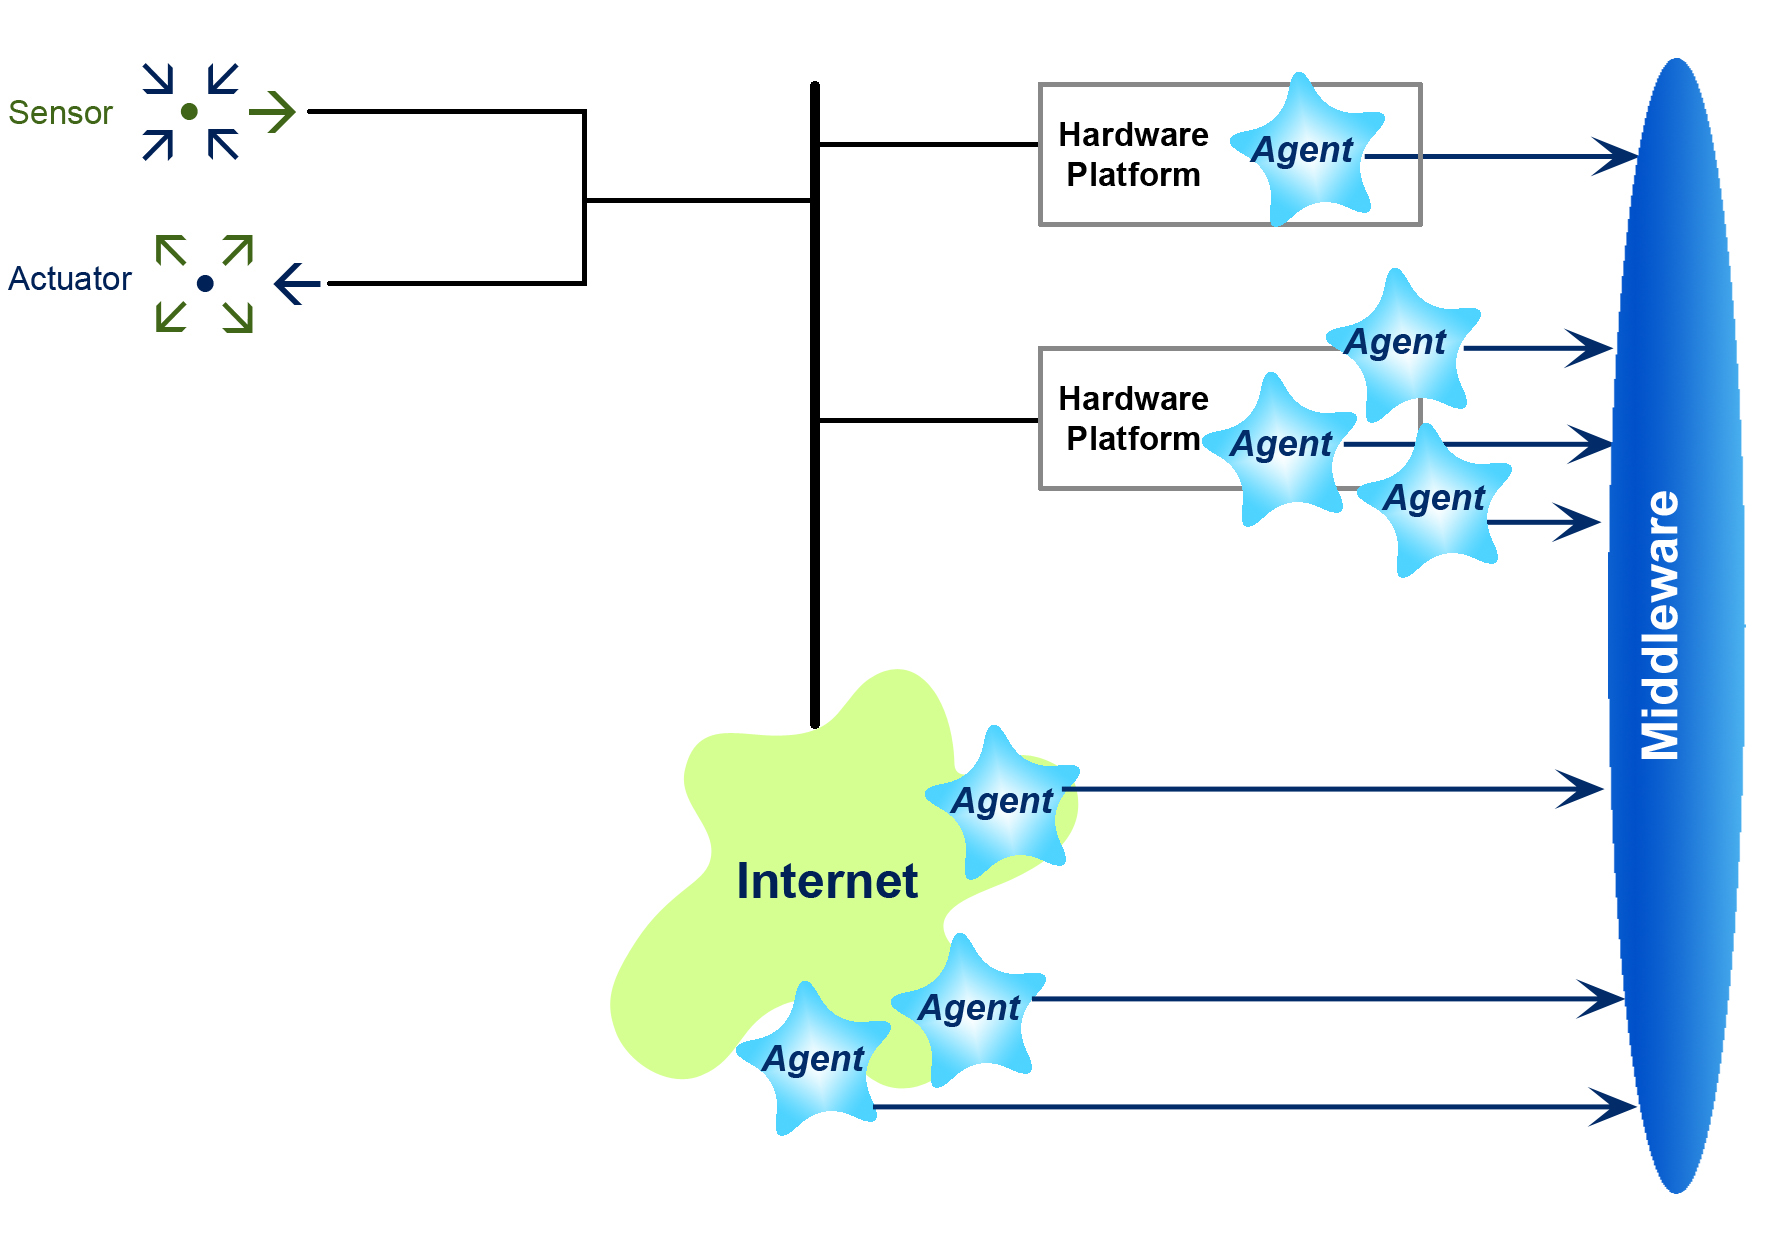
\includegraphics[width=0.9\textwidth, height=0.50\textwidth]{Pic5}
    \caption{The intelligent grid invested with agents. \cite{88} \label{fig:intelligentGridWithAgents}}
\end{figure}

Based on \cref{fig:intelligentGridWithAgents}, the device level contains only sensors and actuators, the connection level contains the middleware,
and the collection level is represented by the agents. With the raise in abstraction level, the hardware aspects lose relevance - the only
relevant aspect are the agents, with the mobility characteristic allowing for the physical components to be changed at any time in order
to suit the problem requirements.

\subsection{Middleware-based simulation for intelligent grid}

The first relevant metric to be measured through simultaneous is the comparison between JADE and conventional middleware. This is done by 
modeling a simple problem to be solved in polynomial time by the same number of nodes in each context. The goal is to measure the time
it takes for the application to complete, using both middlewares. The following graphs showcase the comparison between JADE and typical
middleware (MIP).

?? Fig3.5 ??

?? Fig3.6 ??

From ?? Fig3.5 ?? it can be derived that the time increase in the case of standard middleware follows an exponential curve, due to the 
increase of problem inputs. At the same time, ?? Fig3.6 ?? presents the comparison between MIP and JADE on a constant number of inputs.
The edge gained by the JADE system comes from the implementation using calls for proposal (CFP) - messages sent by agents every time they
require access to a sensor, in order to get its recorded value.

It can be noted that MPI systems are ahead when the node count is low, however they are bottlenecked by the communication overhead after
25 nodes, the point at which the JADE system becomes more efficient. Another significant advantage for JADE is the portability of the code,
allowing for more working environments.

\section{Reliability}

Due to the innate unreliability of disappearing electronics - caused by the ability of grid nodes to emerge, move, fail or running out of
power - designing a reliable system becomes an unavoidable requirement in order to guarantee a secure system. This thesis will address different
means of improving system security and dependability, foremost being the notion of redundancy.

\subsection{Redundancy}

At the connection level, the main concern is the energy consumption of the various sensors and actuators. Although they can be used in a 
myriad of low-power applications, increasing sensor density severely increases the power consumption. An efficient method of combating this 
issue is to create node islands that are powered individually, which are turned off when not in use. While this approach is widely used in 
order to reduce energy consumption, it creates the challenge of introducing complexity into the system - one side-effect could be the creation 
of blind-spots that need to be accounted for. This creates the need for reliable heuristics, meant to maximize area coverage while also 
minimizing power draw \cite{4}.

Redundancy at link level is more challenging, as connection failures cannot be decoupled from component failures. In order to overcome this
particular conundrum, a given component can be linked to several others, thus giving the possibility of determining whether a certain
error was caused by a faulty connection or damaged equipment, while also serving as a mechanism for future fault tolerance. This approach,
however, leads to increased costs, both in terms of wires and communication complexity, but is still a redundancy feature implemented into
the intelligent grid \cite{46}.

An implementation of link level redundancy can be achieved if the controllers and sensors are coupled such that sensors in the same area
are connected to the same controller, with a given amount of overlap between their coverage zone.  Such a design is portrayed in the following:

\begin{figure}[H]
	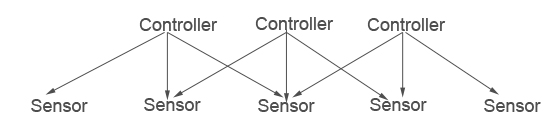
\includegraphics[width=0.9\textwidth, height=0.20\textwidth]{Pic6}
    \caption{Redundancy at link level. \cite{88} \label{fig:redundancy}}
\end{figure}

The type of connection presented in \cref{fig:redundancy} leads to the marginal sensor areas being secluded, however it also causes an 
optimal proportion of redundancy to coverage in the middle section.

Built using the JADE middleware, each controller is managed by an agent that periodically requests the sensor values of all other agents,
using those values to determine an action - in this particular case, setting a variable. The connections were made to be fail-stop, meaning
that if an error occurs, no value is sent. Errors were then introduced, such that they would affect the maximum amount of lines possible,
with the maximum number of errors in which a value from the sensor was received by the controller is given by:

\begin{equation}
    \label{eq:maxErrors}
    max(Errors) = (Full\text{ } covered \text{ } sensonrs) * (Coverage - 1) 
\end{equation}

This architecture implies three independent variables, namely the number of controllers, the number of errors and the sensor redundancy to
coverage proportion. In order to measure performance, the chosen metric was, again, computation time:

?? Fig3.8 ??

In ?? Fig3.8 ??, the variation of compute time is presented in relation to sensor redundancy, with the controller count remaining constant.
It can be noted that the amount of errors introduced is irrelevant for the overall execution time, with the variation being described by:

\begin{equation}
    \label{eq:variationErrors}
    y = \left(a + b * \frac{ln(x)}{x^2} \right)^{-1}
\end{equation}

Relation \cref{eq:variationErrors} is given by the fact that the measure of diversification, \(r^2\), had a maximum value of \(0.9992\) and a 
minimum of \(0.997\), with the error count going from 0 to 7. 

The following figure showcases the results obtained when only a fixed single error is introduced, but the sensor coverage is variable:

?? Fig3.10 ??

As seen in ?? Fig3.10 ??, compute time increases with sensor coverage, with the variation being best described by:

\begin{equation}
    \label{eq:variationCoverage}
    y = (a + b * x^2)
\end{equation}

The final variable to be studied is the controller count, with the following figure showcasing this particular case:

?? Fig3.11 ??

Although incomplete, with portions in which no coverage could be obtained, due to \cref{eq:maxErrors}, from ?? Fig3.11 ?? can be derived 
that the closest approximation is the power function, with \(r^2\) ranging from \(0.993\) to \(0.9999\):

\begin{equation}
    \label{eq:variationControllers}
    y = (a + b * x^c)
\end{equation}

An obvious weakness of this approach appears when attempting to use a wireless network, due to the lack of wires that would provide
redundancy at the link level. A possible solution would be to create message redundancy, such as creating a generic and systematic 
way to transform various agreement problems into consensus, thus creating a unified framework to develop fault-tolerant agreement 
protocols in a modular, correct, and efficient way. An implementation of this principle on the intelligent grid would involve a starting
value for each agent, and a common value that the agents have to agree on. More information can be fount in Versavia Ancusa's PhD report 
\cite{106, 107}.

To conclude, redundancy denotes a correlation between the maximum amount of errors and the minimum amount off sensors for sustainable
system functionality. For this, it is proven that the implementation of the aforementioned redundancy paradigm is a viable solution in
order to maintain a functional system, regardless of possible errors. In summary, sensor area redundancy relates to the devices, the proposed
intelligent grid model implies inter-agent communication, the consensus-based protocol relates to the messages, and the proposed architecture
ensures fault tolerant behavior.

% \cite{3, 4, 8, 9, 19, 23, 24, 30, 32, 33,36, 38, 46, 70, 71, 72, 88, 89, 90}
% \cite{3, 4, 8, 9, 19, 23, 24, 30, 32, 33, 36, 38, 46, 70, 71, 72, 88, 89, 90, 94, 95, 105, 106, 107, 113}
